\chapter{Literature Survey}

1) Authors in \cite{ref1} develop a system to detect brain tumor using Convolutional Neural Network(CNN). The paper mentions the dataset used for training. The same data has been used for the development of the system proposed in this project. The authors mention various other steps implemented which include image augmentation, pre processing, segmentation of the skull, which can be implemented for better training of the model. The authors have used a custom architecture of CNN which provides an efficiency of 95.3\% on test images. The model used by the authors is as follows : 
\begin{figure}[H]
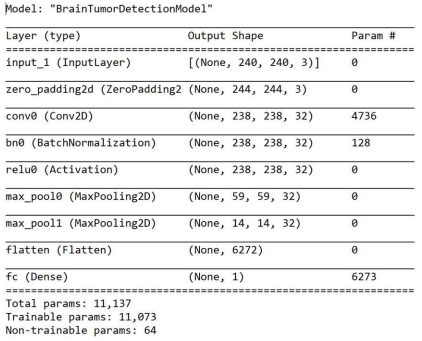
\includegraphics[scale=1]{Photos/paper1_model.PNG}
\caption{Paper 1 Model Summary} \label{fig:ishan}
\end{figure}

2) Authors in \cite{ref2} , \cite{ref3} and \cite{ref5} provides an insight into various symptoms, causes and statistics of brain tumor. This data will be used into the information module of the web application.\\ 

3) Authors in \cite{ref4} provide a survey on major deep learning systems implemented to do various types of brain tumor analysis. This survey gives an insight into the existing detection models. The paper further gives an insight into datasets, techniques into consideration as well as the evaluation of each particular paper considered into the survey.\\

4) Authors in \cite{ref5} use image segmentation as the base technique for detection purpose. The authors use a clustering based approach using Self Organizing Map (SOM) algorithm. The detection works in two phases, the first being image acquisition and pre processing. The second phase is image segmentation which basically segments principle tissue structures in the input images. The authors propose a new MR image segmentation method based on fuzzy C-Means clustering algorithm for the Segmentation which is unsupervised. \\

5) Authors in \cite{ref6} compare nonlinearity reduction with linear method. The authors experiment to check if the non linear method provide better results (unsupervised classification) of MRS brain tumor data. Data reduction is performed using Laplacian eigenmaps (LE) or independent component analysis(ICA). This was then followed by k-means clustering or agglomerative hierarchical clustering (AHC) for unsupervised learning to assess tumor grade and for tissue type segmentation of MRSI data. Based on the results obtained LE method is promising for unsupervised clustering to separate brain and tumor tissue with automated color-coding for visualization of 1 H MRSI data after cluster analysis.\\

6) Authors in \cite{ref7} conduct a survey on different segmentation techniques. The paper provides different papers, their datasets, and various parameter information that gives a brief insight into different algorithms that can be implemented to detect brain tumor. The survey is divided into the following categories: Thresholding techniques, Region growing techniques, Edge based techniques, Clustering techniques, Watershed technique, and Deformable model-based techniques.\\

7) Authors in \cite{ref8} focuses on using image segmentation for brain tumour detection. From the paper it can be inferred that Magnetic Resonance Imaging (MRI) scans are the best medical scan for the training and detection of brain tumour. A deep insight is given into the different parameters associated with image enhancement using different filters and techniques. Furthermore insights are also provided into segmentation techniques.

8) Authors in \cite{ref9} proposed a deep wavelet autoencoder model named "DWAE Model". A high pass filter is used to show the heterogeneity of MRI images. After preprocessing is performed,  the DWAE Model analyzes the pixel pattern of the input scan, and classifies the tumor accordingly. The test results show that the model achieves an accuracy of 99.3\% with a validation loss of 0.1\%.